\documentclass[11pt]{article}
\usepackage[utf8]{inputenc}
\usepackage[dvips]{graphicx}
\usepackage{fancybox}
\usepackage{verbatim}
\usepackage{array}
\usepackage{latexsym}
\usepackage{alltt}
\usepackage{hyperref}
\usepackage{textcomp}
\usepackage{color}
\usepackage{amsmath}
\usepackage{amsfonts}
\usepackage{tikz}
\usepackage{fitch}  % to use fitch
\usepackage{float}
\usepackage[hmargin=3cm,vmargin=5.0cm]{geometry}
%\topmargin=0cm
\topmargin=-2cm
\addtolength{\textheight}{6.5cm}
\addtolength{\textwidth}{2.0cm}
%\setlength{\leftmargin}{-5cm}
\setlength{\oddsidemargin}{0.0cm}
\setlength{\evensidemargin}{0.0cm}


\begin{document}

\section*{Student Information } 
%Write your full name and id number between the colon and newline
%Put one empty space character after colon and before newline
Full Name : Anıl Eren Göçer \\
Id Number : 2448397  \\

\section*{Question 1}

I will use \textbf{Kruskal's Algorithm} in this question. \newline \newline

\noindent \textbf{a)} \newline \newline



\begin{table}[h!]
  \begin{center}
    \label{tab:table1}
    \begin{tabular}{l|c|r} % <-- Alignments: 1st column left, 2nd middle and 3rd right, with vertical lines in between
      \textbf{Adding Order} & \textbf{Edge} & \textbf{Weight}\\
      \hline
      1 & $\{e,f\}$ & 1\\ 
      2 & $\{a,d\}$ & 2\\ 
      3 & $\{g,h\}$ & 2\\
      4 & $\{e,h\}$ & 2\\ 
      5 & $\{d,g\}$ & 3\\ 
      6 & $\{c,f\}$ & 3\\ 
      7 & $\{b,d\}$ & 3\\ 
      8 & $\{h,i\}$ & 4\\ 
    \end{tabular}
  \end{center}
\end{table}

\noindent \textbf{b)} \newline 

\begin{center}
    \textbf{Minimum Spanning Tree Of Graph G}
\end{center}

\begin{center}
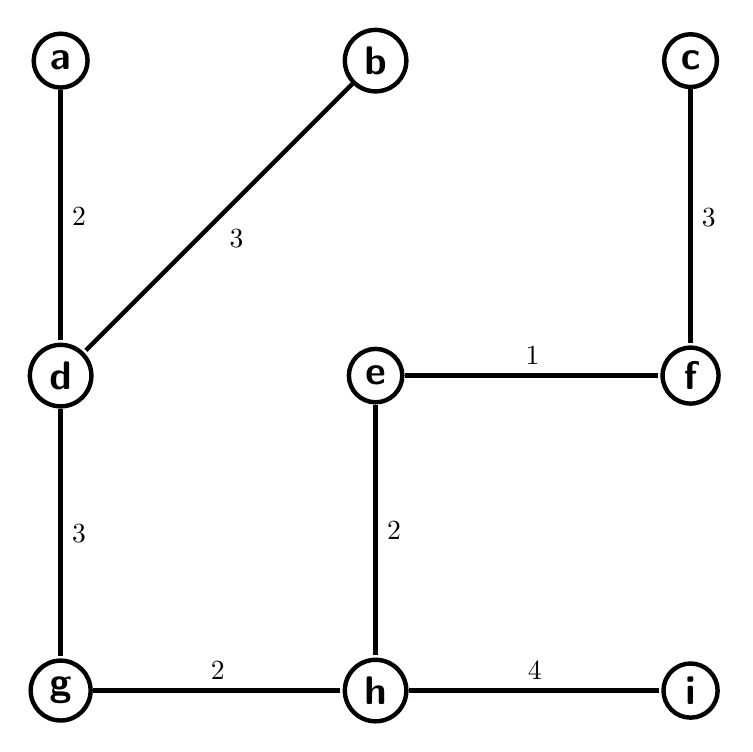
\begin{tikzpicture}[shorten >=1pt, auto, node distance=3cm, ultra thick,
node_style/.style={circle,draw=black,fill=white!20!,font=\sffamily\Large\bfseries},
edge_style/.style={draw=black, ultra thick}]
\node[node_style] (a) at (0,0) {a};
\node[node_style] (b) at (4,0) {b};
\node[node_style] (c) at (8,0) {c};
\node[node_style] (d) at (0,-4) {d};
\node[node_style] (e) at (4,-4) {e};
\node[node_style] (f) at (8,-4) {f};
\node[node_style] (g) at (0,-8) {g};
\node[node_style] (h) at (4,-8) {h};
\node[node_style] (i) at (8,-8) {i};

\draw[edge_style]  (e) edge node{1} (f);
\draw[edge_style]  (a) edge node{2} (d);
\draw[edge_style]  (g) edge node{2} (h);
\draw[edge_style]  (e) edge node{2} (h);
\draw[edge_style]  (d) edge node{3} (g);
\draw[edge_style]  (c) edge node{3} (f);
\draw[edge_style]  (b) edge node{3} (d);
\draw[edge_style]  (h) edge node{4} (i);

\end{tikzpicture}
\end{center}

\newpage
\noindent \textbf{c)} \newline \newline
Answer to the first question (Is the minimum spanning tree unique for the graph G in Figure 1?) : \newline \newline
Yes, the minimum spanning tree for the graph G is unique. \newline
Here is the weights of the minimum spanning tree for the graph G: $\{1,2,2,2,3,3,3,4\}$ . \newline \newline
All edges of weight 1 are included in the minimum spanning tree.  \newline
All edges of weight 2 are included in the minimum spanning tree. \newline \newline

If we could form another MST, we could do it by 
\begin{itemize}
    \item \textbf{Case1: }including the another edge of weight 3 which is $\{f,h\}$ and excluding the edge $\{h,i\}$ which is of weight 4
    \item \textbf{Case2: }including the another edge of weight 3 which is $\{f,h\}$ and excluding the edge $\{b,d\}$ which is of weight 3
    \item \textbf{Case3: }including the another edge of weight 3 which is $\{f,h\}$ and excluding the edge $\{d,g\}$ which is of weight 3
    \item \textbf{Case4: }including the another edge of weight 3 which is $\{f,h\}$ and excluding the edge $\{c,g\}$ which is of weight 3
\end{itemize}
\textbf{But} a circuit (e,h,f) occurs in each case, so these are not spanning trees. Therefore we cannot form another minimum spanning tree. \newline

\noindent Hence, the minimum spanning tree for the graph G is unique. \newline \hline \newline
\noindent \newline Answer to the second question (In general, is the minimum spanning tree unique for any connected edge-weighted undirected graph?): \newline \newline
No, in general, the minimum spanning tree is not unique for any connected edge-weighted directed graph. \newline
If a graph includes edges of the same weight, then this graph \textbf{might} (i.e there is no guarantee) have multiple minimum spanning trees. \newline \newline
For example;
\begin{center}
    \caption{Graph H}
\end{center}
\begin{center}
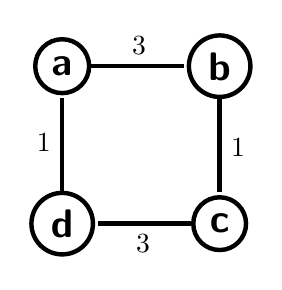
\begin{tikzpicture}[shorten >=1pt, auto, node distance=3cm, ultra thick,
node_style/.style={circle,draw=black,fill=white!20!,font=\sffamily\Large\bfseries},
edge_style/.style={draw=black, ultra thick}]
\node[node_style] (a) at (0,0) {a};
\node[node_style] (b) at (2,0) {b};
\node[node_style] (c) at (2,-2) {c};
\node[node_style] (d) at (0,-2) {d};

\draw[edge_style]  (a) edge node{3} (b);
\draw[edge_style]  (b) edge node{1} (c);
\draw[edge_style]  (c) edge node{3} (d);
\draw[edge_style]  (d) edge node{1} (a);
\end{tikzpicture}
\end{center}
\newpage \noindent the graph H, as given above, has two different minimum spanning trees which are

\begin{center}
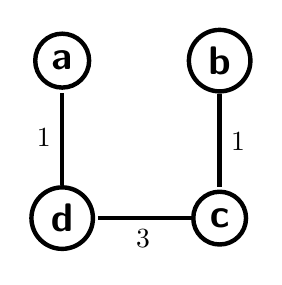
\begin{tikzpicture}[shorten >=1pt, auto, node distance=3cm, ultra thick,
node_style/.style={circle,draw=black,fill=white!20!,font=\sffamily\Large\bfseries},
edge_style/.style={draw=black, ultra thick}]
\node[node_style] (a) at (0,0) {a};
\node[node_style] (b) at (2,0) {b};
\node[node_style] (c) at (2,-2) {c};
\node[node_style] (d) at (0,-2) {d};

\draw[edge_style]  (b) edge node{1} (c);
\draw[edge_style]  (c) edge node{3} (d);
\draw[edge_style]  (d) edge node{1} (a);
\end{tikzpicture}
\end{center}

\newline and

\begin{center}
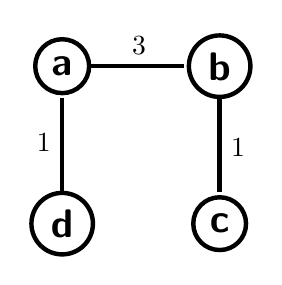
\begin{tikzpicture}[shorten >=1pt, auto, node distance=3cm, ultra thick,
node_style/.style={circle,draw=black,fill=white!20!,font=\sffamily\Large\bfseries},
edge_style/.style={draw=black, ultra thick}]
\node[node_style] (a) at (0,0) {a};
\node[node_style] (b) at (2,0) {b};
\node[node_style] (c) at (2,-2) {c};
\node[node_style] (d) at (0,-2) {d};

\draw[edge_style]  (a) edge node{3} (b);
\draw[edge_style]  (b) edge node{1} (c);
\draw[edge_style]  (d) edge node{1} (a);

\end{tikzpicture}
\end{center}

\newline \noindent Hence, not all connected edge-weighted undirected graphs have unique minimum spanning tree. 
\newline

\hline 
\noindent \newline \textbf{d)} \newline \newline 
\textbf{Proof:} \newline
Let $G$ be a weighted graph and let $e$ be the unique minimum-weight edge of G. \newline \newline
Assume that $T$ is a minimum spanning tree for $G$ which does not contain the edge $e$. \newline \newline
Then consider the graph  $T+e$. This graph must contain a circuit $C$ that contains the edge $e$. \newline \newline
Let $f$ be an edge of C different from $e$, and  \newline \newline
set $T^*$ = $T+e-f$ \newline \newline
Then $T^*$ is also a spanning tree for G, \textbf{but} \newline \newline
$wt(T^*)$ = $wt(T+e-f)$ = $wt(T)$ + $wt(e)$ - $wt(f)$ and $wt(e) < wt(f)$. \newline \newline
This implies $wt(T^*) < wt(T)$, which is an contradiction to T being a minimum spanning tree.  \newline \newline
Therefore, no such minimum spanning tree $T$ (i.e without $e$) can exist. \newline \newline
Hence, for a weighted graph, if the minimum-weight edge pf a graph is unique, then this edge is included in any minimum spanning tree for that graph. 
\newline \newline
(Note that $wt(x)$ gives the weight of the edge x if x is an edge, and gives the total weight of the graph x if x is a graph. )



\newpage
\section*{Question 2}
\noindent Yes, they are isomorphic. \newline \newline
\noindent Let's define an one-to-one and onto function $f$ from the set of vertices $\{a,b,c,d,e,f\}$ to the set of vertices $\{m,n,o,p,r,q\}$ with \newline 

\noindent $f$(a) = n \newline
$f$(b) = q \newline
$f$(c) = o \newline
$f$(d) = r \newline
$f$(e) = m \newline
$f$(f) = p \newline \newline

\noindent Observe that

\begin{itemize}
    \item a is adjacent to the vertices $\{b,d,c\}$ and $f$(a) = n is adjacent to the vertices $f$(b) = q, $f$(d) = r, $f($c) = o.
    \item b is adjacent to the vertices $\{a,c,e,f\}$ and $f$(b) = q is adjacent to the vertices $f$(a) = n, $f$(c) = o, $f($e) = m, $f($f) = p.
    \item c is adjacent to the vertices $\{a,b\}$ and $f$(c) = 0 is adjacent to the vertices $f$(a) = n, $f$(b) = q.
    \item d is adjacent to the vertices $\{a,e\}$ and $f$(d) = r is adjacent to the vertices $f$(a) = n, $f$(e) = m.
    \item e is adjacent to the vertices $\{b,d,f\}$ and $f$(e) = m is adjacent to the vertices $f$(b) = q, $f$(d) = r, $f($f) = p.
    \item f is adjacent to the vertices $\{b,e\}$ and $f$(f) = 0 is adjacent to the vertices $f$(b) = q, $f$(e) = m.
\end{itemize}

\noindent As seen above, for all pairs (x,y), x $\neq$ y in $\{a,b,c,d,e,f\}$, if and only if x and y are connected, $f($x) and $f($y) in $\{m,n,o,p,r,q\}$ are connected . \newline

\noindent Hence, \textbf{$f$ is an isomorphism} . \noindent
\newline \newline
Because $f$ is an isomorphism, graphs $G$ and $H$ are isomorphic.

\newpage

\section*{Question 3}

\textbf{a)}\newline \newline
The number of vertices is \textbf{7}. \newline
The number of edges is \textbf{6}. \newline
The height of T is \textbf{3}. \newline \newline

\noindent \textbf{b)} \newline

\noindent \textbf{postorder: } q,s,u,v,t,r,p \newline \newline
\textbf{inorder: } q,p,s,r,u,t,v \newline \newline
\textbf{preorder:} p,q,r,s,t,u,v  \newline \newline

\noindent \textbf{c)} \newline \newline
\textbf{Yes}, T is a full binary tree because each of its internal vertices (p,r,t) has two children. \newline \newline
\begin{itemize}
    \item p has children q and r
    \item r has children s and t
    \item t has children u,v \newline \newline
\end{itemize}



\noindent \textbf{d)} \newline \newline
\textbf{No}, T is not a complete binary tree.  \newline \newline
For T to be a complete binary tree, it should be completely filled in every level, except possibly the last. And nodes are as far left as. But level 2 of T, i.e level including s:19 and t:43, is not completely filled although it is not the last level. Also, the last level is not filled starting from left. Because of these reasons, T is not a complete binary tree. 

\newpage
\noindent \textbf{e)} \newline \newline
\textbf{No}, T is not a balanced binary tree. \newline \newline
For a binary tree to be balanced, all leaves should be at the levels h and h-1 where h is the last level. \newline \newline
T is not a balanced binary tree because T has a leaf , q:13 , at level 1 which is h-2.  \newline \newline


\noindent \textbf{f)} \newline \newline
\textbf{No}, T is not a binary search tree (BST) . \newline \newline
For a binary tree to be a BST, for each node r in the tree, nodes in the right subtree of the r must have keys greater 
than r's key, and nodes in the left subtree of r must have keys less than the r's key. \newline

\noindent However, for the node r:24, it has u:23 in its right subtree and $23 < 24$, so T is not a BST. \newline \newline

\noindent \textbf{g)} \newline \newline
The minimum number of nodes for a full binary tree with height 5 is \textbf{11}.\newline
The full binary tree of height 5 with minimum number of nodes is in the form of  \newline

\begin{center}
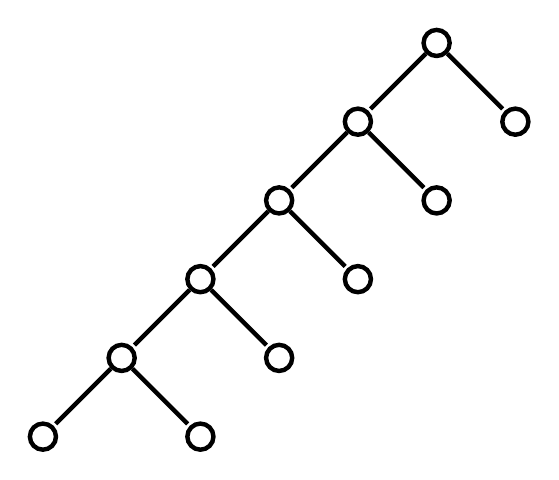
\begin{tikzpicture}[shorten >=1pt, auto, node distance=3cm, ultra thick,
node_style/.style={circle,draw=black,fill=white!20!,font=\sffamily\Large\bfseries},
edge_style/.style={draw=black, ultra thick}]
\node[node_style] (a) at (0,0) {};
\node[node_style] (b) at (-1,-1) {};
\node[node_style] (c) at (1,-1) {};
\node[node_style] (d) at (-2,-2) {};
\node[node_style] (e) at (0,-2) {};
\node[node_style] (f) at (-3,-3) {};
\node[node_style] (g) at (-1,-3) {};
\node[node_style] (h) at (-4,-4) {};
\node[node_style] (i) at (-2,-4) {};
\node[node_style] (j) at (-5,-5) {};
\node[node_style] (k) at (-3,-5) {};

\draw[edge_style]  (a) edge node{} (b);
\draw[edge_style]  (a) edge node{} (c);
\draw[edge_style]  (b) edge node{} (d);
\draw[edge_style]  (b) edge node{} (e);
\draw[edge_style]  (d) edge node{} (f);
\draw[edge_style]  (d) edge node{} (g);
\draw[edge_style]  (f) edge node{} (h);
\draw[edge_style]  (f) edge node{} (i);
\draw[edge_style]  (h) edge node{} (j);
\draw[edge_style]  (h) edge node{} (k);

\end{tikzpicture}
\end{center}

\noindent As seen above, the minimum number of nodes for a full binary tree with height 5 is \textbf{11}.\newline 


\end{document}

 \\